 \documentclass{report}
 
\usepackage[utf8]{inputenc} 
\usepackage[T1]{fontenc}      
\usepackage[top=3.5cm, bottom=3cm, left=3.0cm, right=4.0cm]{geometry}
\usepackage{graphicx}
\graphicspath{{figures/}{../figures}}

\begin{document}

\section*{Exercice 1}

On s'intéresse à l'écoulement stationnaire, incompressible d'un fluide de masse volumique $\rho$ et de viscosité $\eta$ autour d'une sphère de rayon $R$. La vitesse de l'écoulement loin de la sphère est $v_\infty\vec{e_z}$. On adoptera les coordonnées sphériques d'axe $Oz$, $O$ étant le centre le centre de la sphère. 

\begin{itemize}
	\item[•] On suppose que l'écoulement permet de négliger le terme convectif de l'équation de Navier-Stokes devant le terme diffusif. Comment s'écrit alors cette équation ? 
	\item[•] On suppose que la vitesse est telle que : $\vec{rot}(\vec{rot}(\vec{v}))=\frac{3v_\infty R}{r^3}\left(\cos\theta\vec{e_r}+\frac{1}{2}\sin\theta\vec{e_\theta} \right) $. Quelle est la résultante des forces de pression sur la sphère ? 
	\item[•] Quelle est la résultante des actions de cisaillement sur la sphère ? On donne $\left(\frac{\partial v_\theta}{\partial r}\right)_{r=R}=\frac{3v_\infty}{2R}\sin\theta  $.
	\item[•] Trouver la force de trainée s'exerçant sur la sphère. 
\end{itemize}

On donne : 
\begin{equation}
	\Delta f = \frac{1}{r^2}\frac{\partial}{\partial r} \left(r^2\frac{\partial f}{\partial r} \right) + \frac{1}{r^2\sin\theta}\frac{\partial}{\partial \theta} \left(\sin\theta\frac{\partial f}{\partial \theta} \right) + \frac{1}{r^2\sin^2\theta}\frac{\partial^2 f}{\partial \varphi^2} 
\end{equation}

\begin{equation}
	\vec{grad} f = \frac{\partial f}{\partial r} \vec{e_r} + \frac{1}{r}\frac{\partial f}{\partial \theta}\vec{e_\theta} + \frac{1}{r\sin\theta}\frac{\partial f}{\partial \varphi}\vec{e_\varphi}
\end{equation}

\newpage

\section*{Exercice 2}

On considère un fluide d'épaisseur $h$ s'écoulant lentement sur un plan infini incliné d'un angle $\alpha$ par rapport à la verticale. Le fluide a une forte viscosité $\eta$ et une masse volumique $\rho$, et il est soumis à la gravité. On est en régime permanent.

\begin{center}
	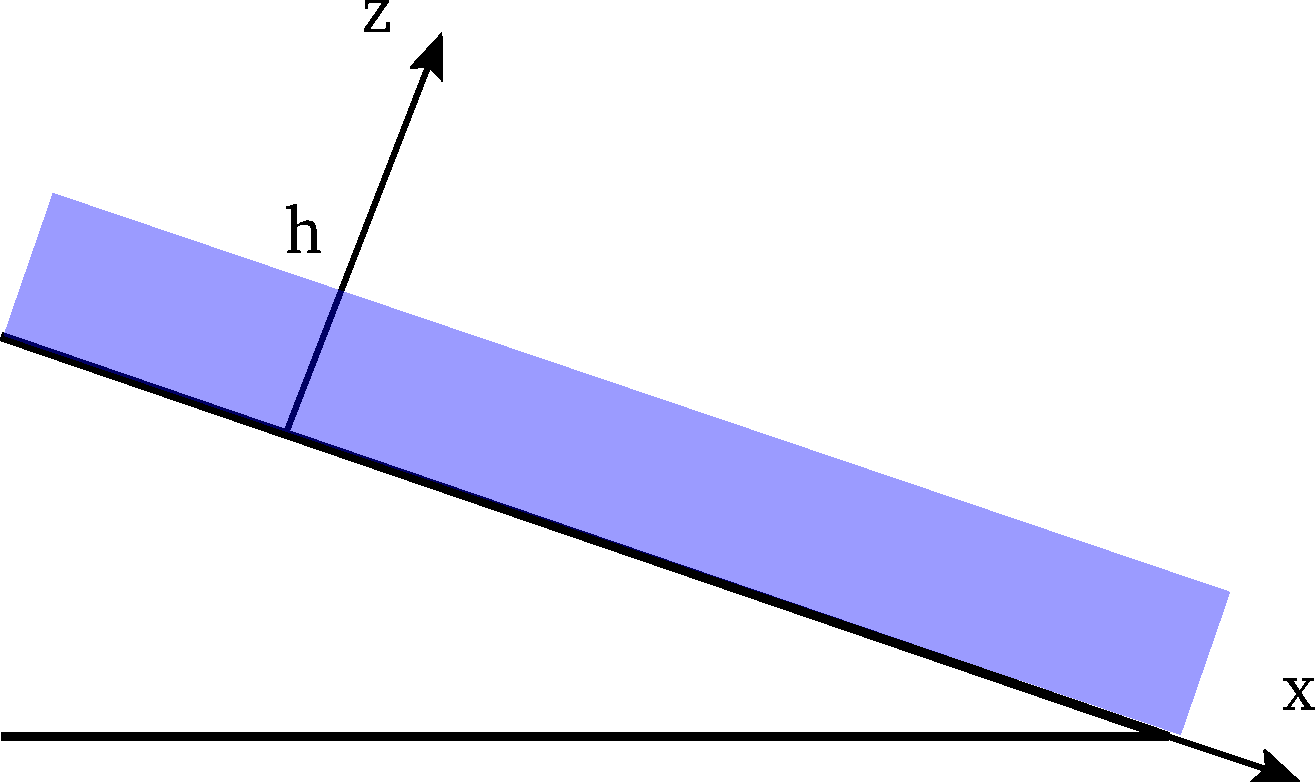
\includegraphics[scale=0.3]{ecoulement.pdf}
\end{center}

\begin{itemize}
	\item[1 -] Quel est le profil de vitesse dans le fluide ? 
	\item[2 -] En déduire le débit. 
	\item[3 -] On observe avec des image satellite que la vitesse d'écoulement d'un glacier à sa surface est d'environ 100m/an. En déduire la viscosité d'un glacier de 100m d'épaisseur, d'un km de large. Quelle quantité de glace est charriée en une année ?
	\item[5 -] On place désormais une plaque au dessus du liquide, au niveau de $z=h$. Que deviennent les conditions aux limites ? Trouver le nouveau profil de vitesse. Comment s'appelle se type d'écoulement ?

\end{itemize}

\end{document}
